\documentclass[11pt]{article} 
\usepackage{setspace}  %line spacing
\usepackage{titling}
\usepackage{siunitx}    %units in maths
\usepackage{graphicx}
\usepackage{parskip}    %spaced paragraphs
\usepackage{csquotes}   %babel wanted it


\usepackage{hyperref}  %have a review of this
\hypersetup{%
  citecolor=black,
  colorlinks=true,
  linkcolor=black,
  urlcolor=black
}

\usepackage{fancyhdr}   %footer
\pagestyle{fancy}
\fancyhf{} % clear existing header/footer entries
\renewcommand{\headrulewidth}{0pt}
% Place Page X of Y on the right-hand
% side of the footer
\fancyfoot[L]{Page \thepage}

\usepackage{pgfgantt}
\setganttlinklabel{s-s}{}
\setganttlinklabel{f-s}{}
\setganttlinklabel{f-f}{}

% \usepackage{tabularx}
\usepackage{booktabs}
% \usepackage{ltablex}
\usepackage{xltabular}
% \usepackage{rotating} 
\usepackage{multirow}
\usepackage{pdflscape}  %pdf support for landscape
% \usepackage{adjustbox}  %table sizing
% \usepackage{lscape}
%  \newcolumntype{b}{>{\hsize=5\hsize}X}
% \newcolumntype{s}{>{\hsize=1.45\hsize}X}
% \newcolumntype{m}{>{\hsize=2.9\hsize}X}

\usepackage[british]{babel} %reduce hyphenation
\renewcommand\britishhyphenmins{60} 

\usepackage{geometry}   %set margins
\geometry{a4paper, margin=2.5cm}

\usepackage{fontspec}
\setmainfont[
    Mapping=tex-text,
    BoldFont={HelveticaNowText-Regular},
    ItalicFont={HelveticaNowText-LightItalic},
    BoldItalicFont={HelveticaNowText-RegIta}
]{[HelveticaNowText-Light]}

\usepackage[
    style=ieee,
    sorting=none
]{biblatex}   %bibliography
\addbibresource{refs.bib}

\usepackage{enumitem}   %reduce list spacing
\setlist{nosep} 



\usepackage{titlesec}   %reduce heading spacing
\titlespacing\section{0pt}{12pt plus 4pt minus 2pt}{0pt plus 2pt minus 2pt}
\titlespacing\subsection{0pt}{12pt plus 4pt minus 2pt}{0pt plus 2pt minus 2pt}
\titlespacing\subsubsection{0pt}{12pt plus 4pt minus 2pt}{0pt plus 2pt minus 2pt}

\setlength{\droptitle}{-4em}     % Eliminate the default vertical space
\addtolength{\droptitle}{-4em}   % Only a guess. Use this for adjustment

\title{\huge Project Feasibility Study\\\Large Portable LoRa Radio Tracker\vspace{0.4em}\\\large 1922268\vspace{-2em}}
% \title{\huge Project Feasibility Study\\\Large Portable LoRa Radio Tracker\\\large}

\preauthor{}
\postauthor{}
\author{}
\predate{}
\date{}
\postdate{}

\begin{document}
\onehalfspacing

\maketitle

\section{Definition}
\subsection{Introduction}
This document is the feasibility study for a LoRa radio based cat tracker.
This project will enable pet owners to allow their pets to roam free where they otherwise would not be able to do so 
(i.e. they live in an apartment and cannot install a catflap).
This has wide reaching potential, with 26\% of UK households owning 11 million cats, of which 63\% spend time outdoors \cite{catsprotection:catsreport}.
Furthermore, the market size for global pet wearables was \$2 billion in 2022 \cite{researchandmarkets:wearablemarket}, proving high demand for such a product. 
Finally, the intended small form-factor and large tracking range make this product potentially applicable 
in many other situations besides the one it is designed to cater for.

\subsection{Aim}
This project will be developing a solution to remotely monitoring a moving,
independent target within a 1km radius of a stationary `base'.
It focuses on cats in particular, however is likely applicable to any ranged moving target.

\subsection{Scope}
Some pets have particularly independent spirits, and perhaps no more renowned for free-roaming prowess is the domestic cat.
Cats are also particularly well known for going missing for days at a time - even years \cite{bbc:missingcat} -, if they return at all.
This project intends to design and develop a product that allows cats to express their natual behaviour \cite{catsprotection:essentialguide} by allowing roaming, 
while providing their owners up-to-date information of their location if, for any reason, it needs to be known.

To achieve this, the cat needs to be fitted with a tracking transmitter of some sort for the period that they are outdoors.
This tracker will transmit location on a regular basis, and will be weather-proof. 
The transmit location will then be received by a permanent fixture at the owner's home, 
after which it can be processed and made presentable, so the cat can be easily located. 

\subsection{Objectives}
This project consists of the following objectives to see completion.
\begin{enumerate}
    \item Obtain ethical approval for experimentation using cats.
    \item Design hardware and software for the tracker.
    \begin{enumerate}
        \item Purchase required hardware.
        \item Develop circuit.
        \item Program the microcontrollers.
        \item Design casing and harness.
    \end{enumerate}
    \item Manufacture the product.
    \item Test reliability and safety.
\end{enumerate}

\subsection{Specification List}
The following specification list dictatest the criteria this project will aim to fulfill.
\begin{itemize}
    \item Portable
    \begin{itemize}
        \item Small form factor (50mm $\times$ 70mm $\times$ 10mm)
        \item Lightweight (<40g)
        \item Battery powered with enough capacity for a day of roaming (\textasciitilde8 hours)
    \end{itemize}
    \item Suitable for home/consumer use
    \begin{itemize}
        \item Installable with tools a consumer could reasonably be expected to own
        \item Compliant to regulations for consumer products
    \end{itemize}
    \item Reliable
    \begin{itemize}
        \item Stable - minimal downtime, if any
        \item Resistant to software and hardware failures
        \item Repairable without great inconvenience or requiring specialised tools
    \end{itemize}
    \item Suitable Reporting
    \begin{itemize}
        \item Regular updates - updates every minute or better
        \item Capable of reporting in any range between 5m and 1000m 
        \item Suited for an urban environment
    \end{itemize}
    \item Safe
    \begin{itemize}
        \item Not a fire hazard
        \item Not an electrocution hazard
        \item Will not cause burns
        \item Comfortable to wear
        \item Compliant with health, safety, data protection, and environmental regulations
    \end{itemize}
\end{itemize}

\subsection{Extensions}
The scope of the project currently only covers location data transmission.
A logical extension would be to render the data in a user-friendly manner.
For example, current and historical location appearing on a map.
With a history of data analysis can be performed, allowing the creation of graphics like heatmaps from location trends. 
Furthermore, if location data is stored (including currently incoming data), 
this can be presented via a webserver such that a user can roam outside and view current location data 
(provided they have an internet connection).

More hardware can be added to the tracker to facilitate enhanced data collection
(accelerometers, piezoelectric sensors, etc.) to recognise activities like types of movement.
A significant feature many trackers utilise is a 'finding' capability of some sort, where the tracker attached to the cat is made to make a noise or flash so it can be found when the owner is within a short range.
This also helps for where a cat returns without the tracker attached, in order to find it again.


\section{Justification}
    The intent of this project is not completely novel. Trackers, in particular for house pets (dogs and cats) and farm cows are commonplace \cite{davcev:lorawan,sivarman:tracker}, 
however these are often based on IoT or LoRaWAN specifically.
The project attempts to introduce a new solution to this existent problem.

Products that achieve similar functionality to the one proposed in this project exist. They can be broken down into two types: 
\begin{itemize}
    \item LTE based - provides completely remote coverage and is only limited by mobile (LTE) network range. These often come with an upfront cost followed by a subscription fee.
    \item RF based - only useable within a limited range. These are often smaller and lighter, but often come with more limited functionality. 
\end{itemize}
The product of this project falls into the latter category, however it benefits from a greatly enhanced range.
LoRa is capable of reliably transmitting over 3km, even in dense suburban areas \cite{augustin:lora}.
In comparison, the Tabcat V2 quotes a range of 152m \cite{tabcat:tracker}. 
While that may be suitable for many owned cats, this does not cover the maximum range an owned cat may roam (278m \cite{hammer:urbanisaton}),
or the typical range of a feral cat (1253m \cite{horn:range}).
Furthermore, a single base will be capable of receiving multiple signals, supporting owners with multiple cats (35\% of cat-owning households \cite{catsprotection:catsreport}).

This product also does not bear reliance on LTE networks, being RF based, and therefore is suitable to use in regions where infrastucture is lacking.
Furthermore, LTE type solutions send and store data to a private server \cite{tractive:privacy}, raising concerns with security and data protection (i.e. an individual's house can be identified from collected location data).

Another style of product uses privately managed networks, built from users of the product (Apple Air Tags, Tile, etc).
This suffers from the same infrastructure problem, except perhaps to a greater degree due to the reliance on distributed consumer use of the product to create the network.

 
\section{Design Overview}

\subsection{Hardware}

There are no specific guidelines on how to approach the hardware design.
The overall circuit is relatively simple and can be built up from individual modules.
However, when using components like microcontrollers off a reel, there comes the issue of programming them.
This requires specialised hardware and writing a bootloader, which is altogether expensive and time-consuming. 
A more cost-effective alternative is to buy hardware with a pre-loaded bootloader, and then lift off the SMD components to create a smaller form factor PCB as necessary.

Microcontroller boards produced by Arduino and Adafruit, to name two, are both cheap and often come with many variations that have additional extras built in.
In the case of the Adafruit M0 LoRa Feather \cite{adafruit:loram0}, a LoRa modulator and ARM M0 microcontroller are both packaged together, along with a serial interface for convenient programming. 

Fabrication of the initial prototype can be done by hand, using breadboards and soldering irons. The final product will have components surface mounted to a PCB, and will at a minimum require a reflow station.

\subsection{Software}
Following the hardware are the software tools used to program the chip. In the case of the Feather, the Arduino IDE \cite{arduino:ide} can be used immediately as compilation libraries for the Feather are provided for this software.
For greater customisation, Assembly, C, or even Rust, can be compiled for the chip, as compilation toolchains exist for all of these. 
However, like with custom hardware, pre-built solutions like the IDE exist to provide a path of least resistance, which is sufficient while the product is in the prototyping stage. 
Developing custom solutions only become viable at the scale of mass production, which is out of the scope of this project. 

\section{Constraints}
\subsection{Security}
This project does not have any security constraints.

\subsection{Intellectual Property}
There currently are no valid UK patents for products that achieve similar goals using the methods described in this feasibility study. 
\subsection{Environment and Sustainability}
This project makes some considerations to sustainability and the right to repair. The casing will be designed in such a way that the user can access the hardware and make minor repairs if necessary. 
No part of the design will intentionally attempt to make repairs difficult. Difficulty only arises in the case of SMD components, for example, which are difficult to work on by hand.

Environmentally, electronics are hazardous and need to be disposed of separately from household waste.
This is especially the case with volatile components like batteries.
As the product is not at the stage of mass production, no specific means of proper disposal have been provided. 
Considerations will be made to make the casing recycleable. 

\subsection{Standards and Legislation}
Short-range radio devices may operate without a commercial license at 868MHz in the UK \cite{ofcom:licenceexempt,ofcom:consultation}.
This is the frequency at which the transmitter will operate.

While this project does not include the scope of commercialisation, the product will aim to adhere to UKCA requirements.
This will require adherence to Electrical Equipment (Safety) Regulations 2016: Great Britain and Radio Equipment Regulations 2017: Great Britain.

\section{Time Management Gantt Chart}
% 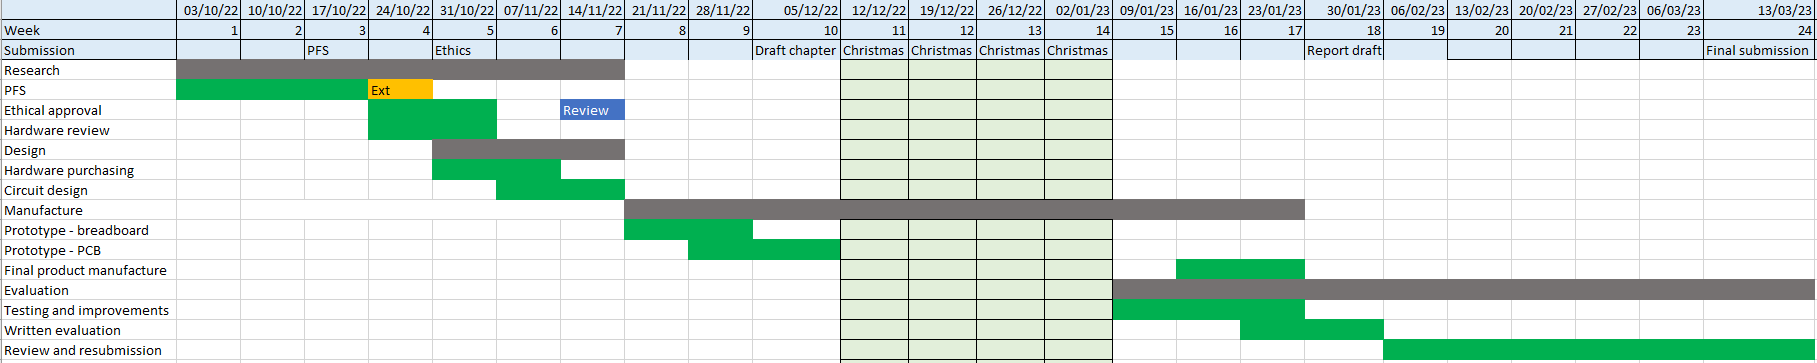
\includegraphics[scale=0.5, angle=90]{./gantt.png}
\begin{ganttchart}[
    hgrid, 
    vgrid,
    bar inline label node/.append style={right=5mm},
    milestone inline label node/.append style={left=5mm}
    ]{1}{25}
    \gantttitle{Term 1}{10} \gantttitle{Christmas}{4} \gantttitle{Term 2}{10} \gantttitle{}{1}\\
    \gantttitlelist{1,...,25}{1} \\

    \ganttgroup{Research}{1}{7} \\
    \ganttbar{PFS}{1}{3} \ganttbar[inline]{Extension}{4}{4} \\
    \ganttbar{Ethical approval}{4}{5} \ganttbar[inline]{Review}{7}{7}\\

    \ganttmilestone[inline, milestone inline label node/.append style={right=5mm}]{Ethics submission}{5} \\
    
    \ganttgroup{Hardware design}{4}{15} \\
    \ganttbar{Hardware review}{4}{4} \ganttbar[inline]{Delivery}{7}{7} \\
    \ganttbar{Circuit design}{5}{5} \\
    \ganttbar{Prototype - breadboard}{6}{8} \\
    \ganttbar{Prototype - PCB}{9}{10} \\
    \ganttbar{Final product}{15}{15} \\

    \ganttgroup{Software design}{4}{15} \\
    \ganttbar{Breadbroad programming}{6}{8} \\
    \ganttbar{PCB programming}{9}{10} \\
    \ganttbar{Final programming}{15}{15} \\

    \ganttmilestone[inline]{Draft chapter}{10} \\

    \ganttgroup{Evaluation}{15}{24} \\
    \ganttbar{Range testing}{15}{16} \\
    \ganttbar{Resistance testing}{15}{16} \\
    \ganttbar{Safety testing}{15}{16} \\
    \ganttbar{Write up}{15}{18} \\
    \ganttmilestone[inline]{Draft submission}{18} \\
    \ganttbar{Improvements}{19}{24} \\

    \ganttmilestone[inline]{Submission}{24}
    
    \ganttlink{elem2}{elem3}    %pfs - ethics
    \ganttlink{elem3}{elem5}    %ethics - sub
    \ganttlink{elem5}{elem4}    %sub - rev
    % \ganttlink{elem3}{elem6}    %ethics - section
    % \ganttlink{elem3}{elem12}   %ethics - section
    \ganttlink{elem7}{elem8}    %hardware review - delivery
    \ganttlink{elem7}{elem9}    %hardware to circuit design
    \ganttlink{elem9}{elem10}   %circuit design - prototype
    \ganttlink{elem10}{elem11}  %proto - proto
    \ganttlink{elem11}{elem12}  %proto - final

    \ganttlink{elem14}{elem15}  %soft proto - proto
    \ganttlink[link mid=0.08]{elem10}{elem14}    %hardware - software
    \ganttlink[link mid=0.91]{elem11}{elem15}   %harware - software
    \ganttlink[link type=s-s]{elem12}{elem16}   %final - final 

    \ganttlink[link type=s-s]{elem19}{elem20}
    \ganttlink[link type=s-s]{elem20}{elem21}
    \ganttlink[link type=s-s]{elem21}{elem22}

    \ganttlink{elem22}{elem23}  %write up - submission
    \ganttlink{elem23}{elem24}  %sub - improv
    \ganttlink{elem24}{elem25}  %improv - final sub
    
\end{ganttchart}
  

\begin{landscape}
\section{Risk Register}
% % \begin{table}[ht]
% \begin{adjustbox}{width=1.8\textwidth,center=\textwidth} 
% \begin{table}[ph!]
% \begin{sidewaystable}[ph!]
\small
% \begin{tabularx}{\columnwidth}{ |m|m|s|s|s|s|b|b| }
% \begin{xltabular}{\linewidth}{ |c|c|X|X|X|X|X|X| }
\begin{xltabular}{1.35\linewidth}{
    |c|
    >{\hsize=1\hsize}X|
    >{\hsize=0.7\hsize}X|
    >{\hsize=0.7\hsize}X|
    >{\hsize=0.6\hsize}X|   
    >{\hsize=0.7\hsize}X|
    >{\hsize=1.8\hsize}X|
    >{\hsize=1.8\hsize}X|
}
\hline
% \multicolumn{8}{|c|}{\large\textbf{Risk Register}} \\

\textbf{Category} & \textbf{Risk Factors} & \textbf{Likelihood \mbox{(out of 10)}} & \textbf{Impact \mbox{(out of 10)}} & \textbf{Total Severity} & \textbf{Risk Status} & \textbf{Risk \mbox{Indicators}} & \textbf{Response}  \\
\hline
\endhead
%Likelihood | Severity  | Total | Status |  Early warning | Actions
\multirow{4}{*}{\textbf{Resources/Financial}} 
& Budget changes            & 1 & 1 & 1  & Safe & Advance notification of budget changes should be received. & Consider alternative funding souces if necessary.  \\ \cline{2-8}
& Overspending              & 1 & 2 & 2  & Safe & Necessary hardware cannot be found within the budget. & Find possible alternatives. Request budget increase.   \\ \cline{2-8}
& Unable to source hardware & 5 & 7 & 35 & Low  & Limited stock in approved vendors. & Prepare alternative options for hardware and vendors. Consider non-approved vendors.  \\ \cline{2-8}
& Data loss                 & 1 & 6 & 6  & Safe & Likely no advance warning possible. & Minimal data held. Any data is held on secured university servers. Backup copies made.  \\ \cline{2-8}
\hline
\multirow{3}{*}{\textbf{Legal/Contractual}}
& Damage            & 2 & 8 & 16 & Low      & Any likelihood of damage will appear during stress testing phase.  & Thorough testing and adherence to electrical/equipment standards.  \\ \cline{2-8}
& Health \& Safety  & 5 & 8 & 40 & Moderate & Health \& safety will be analysed against legislative standards. Any failures of adherence will appear during testing. & Thorough testing and adherence to safety standards.  \\ \cline{2-8}
& IP                & 3 & 3 & 9 & Low       & Project appears too similar to existing IP. & Ensure this project differentiates from existing IP.  \\ \cline{2-8}
\hline
\multirow{2}{*}{\textbf{Method}}
& Equipment issues           & 2 & 8 & 16 & Low          & Equipment availability suffers during course of project. &  Manufacturing up to proof-of-concept can be performed with hand tools. Ensure adequate time management to avoid this. \\ \cline{2-8}
& Manufacturing difficulties & 4 & 7 & 28 & Low-moderate & Manufacturing process is not possible with available equipment or is too difficult to complete to required standard.  & Reconsider utility of chosen manufacturing method and approach alternative ways to achieve same outcome. Ensure competency and training on equipment.\\ \cline{2-8}
& Delays                     & 7 & 7 & 49 & Moderate     & Failure to adhere to Gantt chart. & Ensure project progresses at consistent pace and adheres to outlined schedule.  \\ \cline{2-8}
\hline
\end{xltabular}
% \end{tabularx}
% \end{sidewaystable}
% \end{table}
% \end{tabular}
% \end{adjustbox}
\end{landscape}

\section{Ethics}
\subsection{Animal Ethics}
As the subject of this product will be an animal, the ethics thereof need to be strongly considered. 
The importance of health and safety are paramount, especially given an animal cannot consent to the study. 
The product needs to be safe to wear, and therefore cannot be a fire or electrical hazard, even when caught in poor (especially wet) weather.
Cats may also feel distressed when faced with unfamiliar situations (e.g. when first strapping the harness to the body) which can sometimes be difficult to notice \cite{horowitz:behavioral}. 
This needs to be performed in a safe and ethical manner, such that the animal feels comfortable with the constraints added to their body by way of gentle, gradual introduction. 
Further considerations need to be made to ensure the harness is comfortable to wear for long periods of time, and that it is not heavy, digs in, or otherwise burdensome. 
\subsection{Human Ethics}
The normal scope of the project does not require experimentation on people.
\subsection{Environmental and Social Ethics}
The normal scope of the project does not face environmental or social issues.

\printbibliography
\end{document}
